\documentclass{beamer}
\let\Tiny=\tiny %to avoid warnings related to font size and beamer 
\usetheme{Amsterdam}
\usecolortheme{dolphin}
\usepackage{amsmath}
\usepackage{tikz}
\usepackage{verbatim}
\usetikzlibrary{arrows,shapes}
\usepackage{hyperref}
\usepackage[style=verbose,backend=bibtex]{biblatex}
\usepackage{comment}
\usepackage{listings}
\usepackage{algorithm}
\usepackage{algpseudocode}

\addbibresource{../sources}

\let\oldfootnotesize\footnotesize
\renewcommand*{\footnotesize}{\oldfootnotesize\tiny}

\title{Parallel network flows}
\subtitle{A follow up seminar to the Parallel Algorithms lecture}
\author{Martin Kalany\inst{1} }
\institute
{
  \inst{1}
  Graduate student in Computer Science\\
  Vienna University of Technology\\
}
\date{\today}

\AtBeginSection[]
{
  \begin{frame}
    \frametitle{Table of Contents}
    \tableofcontents[currentsection]
  \end{frame}
}

\tikzstyle{vertex}=[circle,fill=black!25,minimum size=20pt,inner sep=0pt]
\tikzstyle{edge} = [draw,thick,->,>=latex,shorten >=1pt]
\tikzstyle{weight} = [font=\small]
\tikzstyle{selected edge} = [draw,line width=2pt,->,red!75,>=latex]
\tikzstyle{residual edge} = [draw,thick,->,blue!75,>=latex]
\tikzstyle{vertexE}=[circle,fill=black!25,minimum size=20pt,inner sep=0pt]


\begin{document}
% Declare layers (for more convenience when drawing graphs)
\pgfdeclarelayer{background}
\pgfsetlayers{background,main}

\frame{\titlepage}
	
\section{Network flows}
\begin{frame}
	\frametitle{Network flows}
    \begin{block}{Definition: Flow network}\footnote{\cite{ahuja93}}
    A \textcolor{red}{flow network}  is given by $N = (G,s,t,c)$, where
    \begin{itemize}
    		\item $G =(V,A)$ is a directed graph
    		\item $s$ and $t$, $s \neq t$ are the source and terminal node
    		\item $c:A\rightarrow \mathbb{R}_0^{+}$ assigns a capacity $\forall a \in A$
    \end{itemize}
    \end{block}
    \textbf{Assumptions:}
	\begin{itemize}
		\item $G$ is connected
		\item $\nexists P(s,t) \in G$ s.t. $c(P) = \infty$
		\item $G$ is simple, i.e., does not contain loops or parallel arcs
	\end{itemize}
\end{frame}
  
\begin{frame}[shrink]
	\frametitle{Network flows}
	\begin{block}{Definition: Flow}
	$f:A \rightarrow \mathbb{R}_0^{+}$ is a \textcolor{red}{flow} if it satisfies:
	\begin{itemize}
		\item \textbf{Capacity constraints:} $f(a) \leq c(a)$ $\forall a \in A$
		\item \textbf{Flow conservation:} 
		$ \sum\limits_{v \in V} f(u,v) =  0 \Leftrightarrow IN(f,v) = OUT(f,v)$ $\forall v \in V \setminus \{s,t\}$
		\item \textbf{Value of a flow:} $\lvert f\rvert = f(V,t)$ 
	\end{itemize}
	\end{block}
	
	\begin{block}{A flow $f$}
	\begin{itemize}
		\item is a \textcolor{red}{maximum flow} if $\lvert f\rvert \geq \lvert f'\rvert$, for any other flow $f'$
		\item \textcolor{red}{saturates} an arc a if $f(a) = c(a)$
		\item is a \textcolor{red}{maximal (or blocking) flow} if every directed path P(s,t) contains at least one saturated edge
	\end{itemize}
	\end{block}
\end{frame}

\begin{frame}
	\frametitle{Network flows}
	\begin{block}{Definition: Residual capacity}
		The \textcolor{red}{residual capacity} of $a \in V \times V$ w.r.t. a flow $f$ is defined as $r_f(a) = c(a) - f(a)$. \\
	\end{block}
	
	\pause
	\begin{block}{Definition: Residual network}
		$G_r = (V, A_r)$ with $A_r = \left\{a \in V \times V \lvert r_f(a) > 0\right\}$
	\end{block}
	
	\pause
	\begin{block}{Definition: Augmenting path}
		A path $P$ from $s$ to $t$ in $G_r$ is called an \textcolor{red}{augmenting} path and can be used to increase the flow $f$.
	\end{block}
\end{frame}


\section{Ford-Fulkerson}
\begin{frame}
	\frametitle{Algorithm of Ford-Fulkerson}
	\framesubtitle{An intuitive sequential algorithm}
	
	\visible<1-2>{
	\begin{figure}
	\begin{tikzpicture}[scale=1.8, auto,swap]
    	% draw the vertices
	    \foreach \pos/\name in {{(0,2)/s}, {(1,3)/v_1}, {(2.5,3)/v_2},
    	                        {(1,1)/v_3}, {(2.5,1)/v_4}, {(3.5,2)/t}}
        \node[vertex] (\name) at \pos {$\name$};
    	% Connect vertices with edges and draw weights
    	\foreach \source/ \dest /\weight in {s/v_1/2, s/v_3/8,v_3/v_1/5,
                                         v_1/v_2/7, v_4/v_2/15, v_3/v_4/5,
                                         v_2/t/2, v_4/t/5}
        	\path[edge] (\source) -- node[weight] {$\weight$} (\dest);
        	
        	%v_1/v_4/9
        	\path[edge] ([xshift= -2pt, yshift= 5pt] v_4.center) -- node[weight] {6}  ([xshift= 5pt, yshift= -2pt] v_1.center);
        	\path[edge] ([xshift = 2pt, yshift= -5pt] v_1.center) -- node[weight] {9}  ([xshift= -5pt, yshift= 2pt] v_4.center);
  
	    % For convenience we use a background layer to highlight edges
    	% This way we don't have to worry about the highlighting covering
	    % weight labels. 
	    \begin{pgfonlayer}{background}
	        \pause
    	    \foreach \source /\dest  /\weight in {s/v_3/5,v_4/t/5}
	            \path[selected edge] (\source) -- node[weight,above] {$\weight$}(\dest);		
	            \path[selected edge] ([xshift = 2pt, yshift= -5pt] v_1.center) -- node[weight,left] {5}  ([xshift= -5pt, yshift= 2pt] v_4.center);
	            \path[selected edge] (v_3) -- node[weight,left] {$5$}(v_1);
    	\end{pgfonlayer}
	\end{tikzpicture}
	\end{figure}
	}	
\end{frame}

\begin{frame}
	\frametitle{Algorithm of Ford-Fulkerson}
	\framesubtitle{An intuitive sequential algorithm}

	\begin{figure}
	\begin{tikzpicture}[scale=1.8, auto,swap]
    	% draw the vertices
	    \foreach \pos/\name in {{(0,2)/s}, {(1,3)/v_1}, {(2.5,3)/v_2},
    	                        {(1,1)/v_3}, {(2.5,1)/v_4}, {(3.5,2)/t}}
        \node[vertex] (\name) at \pos {$\name$};
    	% Connect vertices with edges and draw weights
    	\foreach \source/ \dest /\weight in {s/v_1/2, v_1/v_3/5, t/v_4/5,
                                         v_1/v_2/7, v_4/v_2/15, v_3/v_4/5,
                                         v_2/t/2}
        	\path[residual edge] (\source) -- node[weight] {$\weight$} (\dest);

        	%s/v_3/8,
        	\path[residual edge] ([xshift= -2pt, yshift= 5pt] v_3.center) -- node[weight] {5}  ([xshift= 5pt, yshift= -2pt] s.center);
        	\path[residual edge] ([xshift = 2pt, yshift= -5pt] s.center) -- node[weight] {3}  ([xshift= -5pt, yshift= 2pt] v_3.center);
        	%v_1/v_4/9
        	\path[residual edge] ([xshift= -2pt, yshift= 5pt] v_4.center) -- node[weight] {11}  ([xshift= 5pt, yshift= -2pt] v_1.center);
        	\path[residual edge] ([xshift = 2pt, yshift= -5pt] v_1.center) -- node[weight] {4}  ([xshift= -5pt, yshift= 2pt] v_4.center);       	
        	
        	\begin{pgfonlayer}{background}
	        \pause
    	    \foreach \source /\dest  /\weight in {s/v_1/2,v_1/v_2/2,v_2/t/2}
	            \path[selected edge] (\source) -- node[weight,above] {$\weight$}(\dest);			            
    	\end{pgfonlayer}
	\end{tikzpicture}
	\end{figure}
		
\end{frame}		


\begin{frame}
	\frametitle{Algorithm of Ford-Fulkerson}
	\framesubtitle{An intuitive sequential algorithm}

	\begin{figure}
	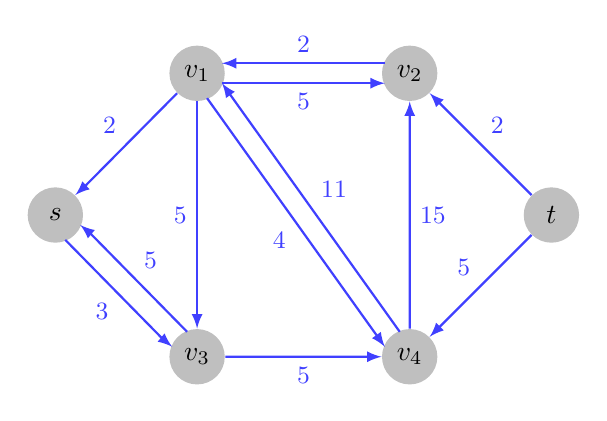
\begin{tikzpicture}[scale=1.8, auto,swap]
    	% draw the vertices
	    \foreach \pos/\name in {{(0,2)/s}, {(1,3)/v_1}, {(2.5,3)/v_2},
    	                        {(1,1)/v_3}, {(2.5,1)/v_4}, {(3.5,2)/t}}
        \node[vertex] (\name) at \pos {$\name$};
    	% Connect vertices with edges and draw weights
    	\foreach \source/ \dest /\weight in {v_1/s/2, v_1/v_3/5, t/v_4/5,
                                         v_4/v_2/15, v_3/v_4/5,
                                         t/v_2/2}
        	\path[residual edge] (\source) -- node[weight] {$\weight$} (\dest);

        	%s/v_3/8,
        	\path[residual edge] ([xshift= -2pt, yshift= 5pt] v_3.center) -- node[weight] {5}  ([xshift= 5pt, yshift= -2pt] s.center);
        	\path[residual edge] ([xshift = 2pt, yshift= -5pt] s.center) -- node[weight] {3}  ([xshift= -5pt, yshift= 2pt] v_3.center);
        	%v_1/v_4/9
        	\path[residual edge] ([xshift= -2pt, yshift= 5pt] v_4.center) -- node[weight] {11}  ([xshift= 5pt, yshift= -2pt] v_1.center);
        	\path[residual edge] ([xshift = 2pt, yshift= -5pt] v_1.center) -- node[weight] {4}  ([xshift= -5pt, yshift= 2pt] v_4.center);       	
			%v_1/v_2/7
        	\path[residual edge] ([xshift= 5pt, yshift= -2pt] v_1.center) -- node[weight] {5}  ([xshift= -5pt, yshift= -2pt] v_2.center);
        	\path[residual edge] ([xshift = -5pt, yshift= 2pt] v_2.center) -- node[weight] {2}  ([xshift= 5pt, yshift= 2pt] v_1.center);               		
	\end{tikzpicture}
	\end{figure}
\end{frame}		

\begin{frame}
	\frametitle{Algorithm of Ford-Fulkerson}
	\framesubtitle{An intuitive sequential algorithm}
	
	\begin{columns}[c] 
    \column{.5\textwidth} 
	\begin{figure}
	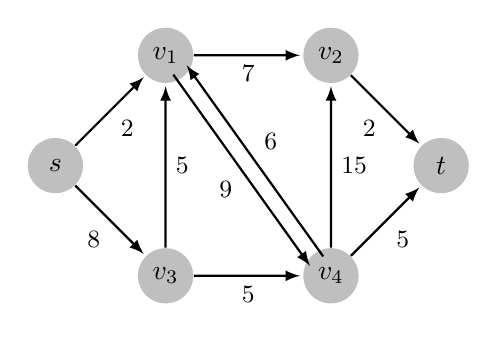
\begin{tikzpicture}[scale=1.4, auto,swap]
    	% draw the vertices
	    \foreach \pos/\name in {{(0,2)/s}, {(1,3)/v_1}, {(2.5,3)/v_2},
    	                        {(1,1)/v_3}, {(2.5,1)/v_4}, {(3.5,2)/t}}
        \node[vertex] (\name) at \pos {$\name$};
    	% Connect vertices with edges and draw weights
    	\foreach \source/ \dest /\weight in {s/v_1/2, s/v_3/8,v_3/v_1/5,
                                         v_1/v_2/7, v_4/v_2/15, v_3/v_4/5,
                                         v_2/t/2, v_4/t/5}
        	\path[edge] (\source) -- node[weight] {$\weight$} (\dest);
        	
        	%v_1/v_4/9
        	\path[edge] ([xshift= -2pt, yshift= 5pt] v_4.center) -- node[weight] {6}  ([xshift= 5pt, yshift= -2pt] v_1.center);
        	\path[edge] ([xshift = 2pt, yshift= -5pt] v_1.center) -- node[weight] {9}  ([xshift= -5pt, yshift= 2pt] v_4.center);	 
	\end{tikzpicture}
	\end{figure}
    \column{.5\textwidth}
	\begin{figure}
	\begin{tikzpicture}[scale=1.4, auto,swap]
    	% draw the vertices
	    \foreach \pos/\name in {{(0,2)/s}, {(1,3)/v_1}, {(2.5,3)/v_2},
    	                        {(1,1)/v_3}, {(2.5,1)/v_4}, {(3.5,2)/t}}
        \node[vertex] (\name) at \pos {$\name$};
    	
	    \begin{pgfonlayer}{background}
    	    \foreach \source /\dest  /\weight in {s/v_3/5,v_4/t/5,s/v_1/2,v_1/v_2/2,v_2/t/2}
	            \path[selected edge] (\source) -- node[weight,above] {$\weight$}(\dest);		
	            \path[selected edge] ([xshift = 2pt, yshift= -5pt] v_1.center) -- node[weight,left] {5}  ([xshift= -5pt, yshift= 2pt] v_4.center);
	            \path[selected edge] (v_3) -- node[weight,left] {$5$}(v_1);
    	\end{pgfonlayer}
	\end{tikzpicture}
	\end{figure}
    \end{columns}	
\end{frame}


\section{Computational Complexity}
\begin{frame}
	\frametitle{Computational Complexity}
	\begin{itemize}
		\item Sequential complexity:
		\begin{itemize}
			\item Ford-Fulkerson: $O((|A|+|V|)*f_{max})$
			\item Edmonds-Karp: $O(|V|^{2} * |E|) $
			\pause \\	
			$\Rightarrow$ \textcolor{green}{clearly solvable in polynomial time}
		\end{itemize}
		\pause
		\item Parallel complexity:
		\begin{itemize}
			\item Construct residual network: $O(1)$
			\item Find augmenting path: $O(log^{2}|V|)$ time and $O(|V|^{2})$ work
			\item Number of stages: $O(|f_{max}|)$\\
			may be reduced\footcite{papa95} to $O(|V|)$ or even $O(\sqrt{|V|})$
		\end{itemize}			
		\pause
		\textcolor{blue}{Can we get an "efficient" parallel algorithm?}
	\end{itemize}
\end{frame}

\begin{frame}
	\frametitle{Computational Complexity}
	\begin{itemize}
	\item \textbf{NC}\footcite{papa95} ("Nick's Class"): Problems solvable in $O(log^{k_1}(n))$ time and $O(n^{k_2})$ total work
	\item alternatively: Language decided by PRAM in $O(log^{k_1}(n))$ time steps with $O(n^{k_2})$ processors available at each step 
	\item $NC \subseteq P$, but whether $NC \subset P$ or $NC = P$ is unknown 
	\item $P \setminus NC$: "Inherently sequential"  problems
	\item Most likely candidates to be in $P \setminus NC$: P-complete problems
	\end{itemize}

	\pause	
	\textcolor{red}{Max-flow is P-complete.} \\
	No parallel algorithm to solve the problem in poly-log time is currently known.	
\end{frame}

\section{Parallel algorithms}
\subsection{Dinitz' scheme}
\begin{frame}
\frametitle{Dinitz' scheme}
	

	
	\begin{block}{Lemma: Dinitz' scheme\footcite{dinitz70}}
	A maximum flow problem in a \emph{general network} can be transformed \emph{into $O(n)$ maximal flow problems in layered networks}.
	\end{block}
\end{frame}

\begin{frame}[shrink]

\frametitle{Layered networks}
	\begin{block}{Definition: Layered network\footcite{yossi81}}
	$N = (V,A,s,t,c)$ is a \textcolor{red}{layered network} if each vertex $v \in V$ has a layer number $l(v)$ s.t.
	\begin{itemize}
		\item $l(s) = 0$ and $0 \leq l(v) \leq l(t)$ $\forall v \in V$
		\item $(e = u \rightarrow v) \in A  \Rightarrow l(v) - l(u) = 1$
	\end{itemize}
	\end{block}
	
\begin{figure}
	\begin{tikzpicture}[scale=1.2, auto,swap]
    	% draw the vertices
	    \foreach \pos/\name/\layer in {{(0,2)/s/0}, {(1,3)/v_1/1}, {(2.5,3)/v_2/2},
    	                        {(1,1)/v_3/1}, {(2.5,1)/v_4/2}, {(3.5,2)/t/3}}
        \node[vertex,label={[color=blue]80:$\layer$}] (\name) at \pos {$\name$};
        
        %\node[vertex,label={[color=blue]80:$+12$}] (v_1) at (1.5,3) {$v_1$};
    	% Connect vertices with edges and draw weights
    	\foreach \source/ \dest in {s/v_1, s/v_3,v_3/v_1,
                                         v_1/v_2, v_4/v_2, v_3/v_4,
                                         v_2/t, v_4/t}
        	\path[edge] (\source) -- (\dest);
        	
        	%v_1/v_4/9
        	\path[edge] ([xshift= -2pt, yshift= 5pt] v_4.center) -- ([xshift= 5pt, yshift= -2pt] v_1.center);
        	\path[edge] ([xshift = 2pt, yshift= -5pt] v_1.center) -- ([xshift= -5pt, yshift= 2pt] v_4.center);
  
	    % For convenience we use a background layer to highlight edges
    	% This way we don't have to worry about the highlighting covering
	    % weight labels. 
	    \begin{pgfonlayer}{background}
    	    \foreach \source /\dest in {s/v_3,v_2/t,s/v_1,v_1/v_2}
	            \path[selected edge, color=blue] (\source) -- (\dest);		
	            \path[selected edge, color=blue] ([xshift = 2pt, yshift= -5pt] v_1.center) -- ([xshift= -5pt, yshift= 2pt] v_4.center);
	    \end{pgfonlayer}
	\end{tikzpicture}
	\end{figure}

\end{frame}

\subsection{Algorithm 1}
\begin{frame}
\frametitle{Algorithm 1}
\framesubtitle{Shiloach and Vishkin\footcite{yossi81}} 

	\begin{algorithmic}[5]
		\State Input: Flow network $N=(V,A,s,t,c)$
		\State start with some valid flow 
		\While{$\neg$ finished} \Comment{$O(\lvert V \rvert)$}
			\State Construct residual network $G_r$ \Comment{$O(\lvert V \rvert)$, $p=O(\lvert V \rvert)}$
			\State Construct layered network $G_l$ from $G_r$ \Comment{$O(\lvert A \rvert/p + \lvert V \rvert)$ (BFS on CREW)}
			\State Calculate max flow $f_l$ in $G_l$  \Comment{next slides}
			\State $f$ = $f$ + $f_l$
		\EndWhile	
	\end{algorithmic}
\end{frame}

\begin{frame}
\frametitle{Algorithm 1}
\framesubtitle{Shiloach and Vishkin\footcite{yossi81}} 
\end{frame}

\begin{comment}
Preflow push on layered network
implementation details (?)
only n processors (just state)
2n bound proof
\end{comment}

\begin{frame}
\frametitle{Algorithm 1}
\framesubtitle{Problems in acyclic networks\footcite{vishkin92}} 
\end{frame}

\begin{comment}
Just mention briefly
\end{comment}

\subsection{Algorithm 2}
\begin{frame}
\frametitle{Algorithm 2}
\framesubtitle{Goldberg and Tarjan\footcite{goldberg89}} 
\end{frame}
\begin{comment}
Atomic method
proof (?)
\end{comment}



\begin{comment}
\section{Preflow-Push}
\begin{frame}
	\frametitle{Preflow-Push Algorithm}
	\begin{itemize}
		\item Push flow along individual arks instead of paths from $s$ to $t$
		\item Excess flow $e_f(v) \geq 0$ $\forall v \in V$\\
	\end{itemize}

	\begin{figure}
	\begin{tikzpicture}[scale=1.8, auto,swap]
    	% draw the vertices
	    \foreach \pos/\name in {{(0,2)/s}, {(1.5,3)/v_1}, {(3,3)/v_2},
    	                        {(1.5,1)/v_3}, {(3,1)/v_4}, {(4.5,2)/t}}
        \node[vertex] (\name) at \pos {$\name$};
    	% Connect vertices with edges and draw weights
    	\foreach \source/ \dest /\weight in {s/v_1/12, s/v_3/11,v_3/v_1/5,v_1/v_4/9,
                                         v_1/v_2/7, v_4/v_2/15, v_3/v_4/5,
                                         v_2/t/8, v_4/t/9}
        	\path[edge] (\source) -- node[weight] {$\weight$} (\dest);
        	\path[edge] (v_4) to[bend right] node[weight] {6}  (v_1);
  
	    % For convenience we use a background layer to highlight edges
    	% This way we don't have to worry about the highlighting covering
	    % weight labels. 
	    \begin{pgfonlayer}{background}
	        \pause
    	    \foreach \source /\dest  /\weight in {s/v_3/11,s/v_1/12}
	            \path[selected edge] (\source) -- node[weight,above] {$\weight$} (\dest);
	            \node[vertex,label={[color=blue]80:$+12$}] (v_1) at (1.5,3) {$v_1$};
	            \node[vertex,label={[color=blue]280:$+11$}] (v_3) at (1.5,1) {$v_3$};
	           

    	\end{pgfonlayer}
	\end{tikzpicture}
	\end{figure}	
\end{frame} 
\end{comment}
 	 
\begin{frame}[allowframebreaks]
\frametitle<presentation>{Literature}    
\printbibliography
\end{frame} 	 
 	 
\end{document}